\documentclass{beamer}

%%%%%%%%%%%%%Solarized Theme%%%%%%%%%%%%%%%
\usecolortheme[dark,accent=cyan]{solarized}
\beamertemplatenavigationsymbolsempty
%%%%%Packages%%%%%
\usefonttheme{serif}
\usepackage[T1]{fontenc}
\usepackage[utf8]{inputenc}
\usepackage[english]{babel}
\usepackage{fontawesome}
\usepackage{minted}
\usepackage{media9}
\usepackage{multimedia}
\usepackage{animate}

\definecolor{DarkGray}{gray}{0.1}
\usemintedstyle{paraiso-dark}


\usepackage{graphicx}
\usepackage{hyperref}
\usepackage{colortbl, xcolor}
\usepackage{booktabs}
\usepackage{amsmath,amsthm, amssymb, latexsym}

\usepackage{tikz}
\usepackage{standalone}
\usepackage{siunitx}
\usetikzlibrary{calc, positioning, arrows, arrows.meta, shapes}
\usetikzlibrary{backgrounds, fit}
\makeatletter
\newcommand{\srcsize}{\@setfontsize{\srcsize}{5pt}{5pt}}
\makeatother

\begin{document}

\begin{frame}
    \begin{center}
        \LARGE{\textbf{\textcolor{orange}{THE FALLACY OF MERITOCRACY}}} \\

        \vspace{1.5cm}
        \normalsize{PyCon Balkan}

        \vspace{1cm}
        \normalsize{@NikoletaGlyn}

    \end{center}
\end{frame}

\begin{frame}
    \begin{center}
    
\includegraphics[width=0.24\textwidth]{static/cardiff_uni_logo.png}\hspace{6pt}
    
\includegraphics[width=0.24\textwidth, height=0.245\textwidth]{static/django_girls.png}\vspace{10pt}

    
\includegraphics[width=0.24\textwidth]{static/ssi-logo.png} \hspace{6pt}
    
\includegraphics[width=0.24\textwidth]{static/plos-logo.jpg}

    \end{center}
\end{frame}

\begin{frame}
    \begin{center}
    
\includegraphics[width=0.24\textwidth]{static/shake.png} \hspace{6pt}
    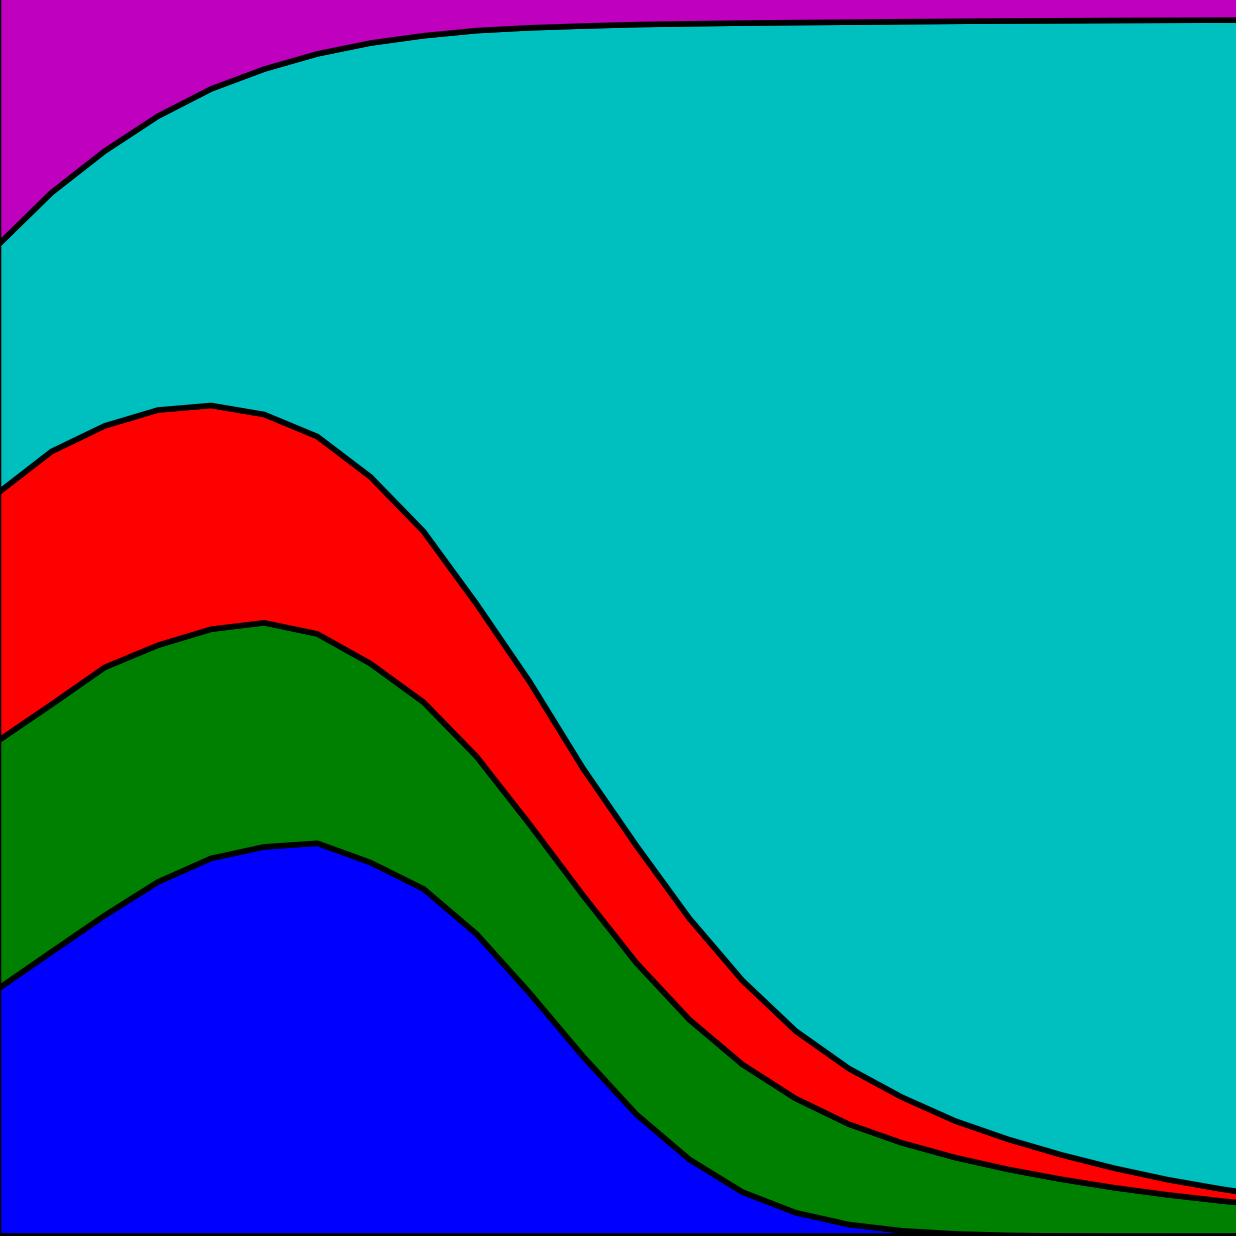
\includegraphics[width=0.24\textwidth]{static/axelrod-logo.png}

    \end{center}
\end{frame}

\begin{frame}
    \begin{center}
    \begin{minipage}{.5\textwidth}
        \LARGE{MERITOCRACY}
    \end{minipage}
    \begin{minipage}{.3\textwidth}
        \normalsize{[mer-i-tok-ruh-see]}
    \end{minipage}
    \vspace{.5cm}

    \hspace{-8cm} \normalsize{[noun]}\\
    \end{center}
    \hspace{.8cm} \normalsize{1. government or the holding of power by people}

    \hspace{1cm}\normalsize{selected according to merit.}
\end{frame}

\begin{frame}
    \begin{center}
    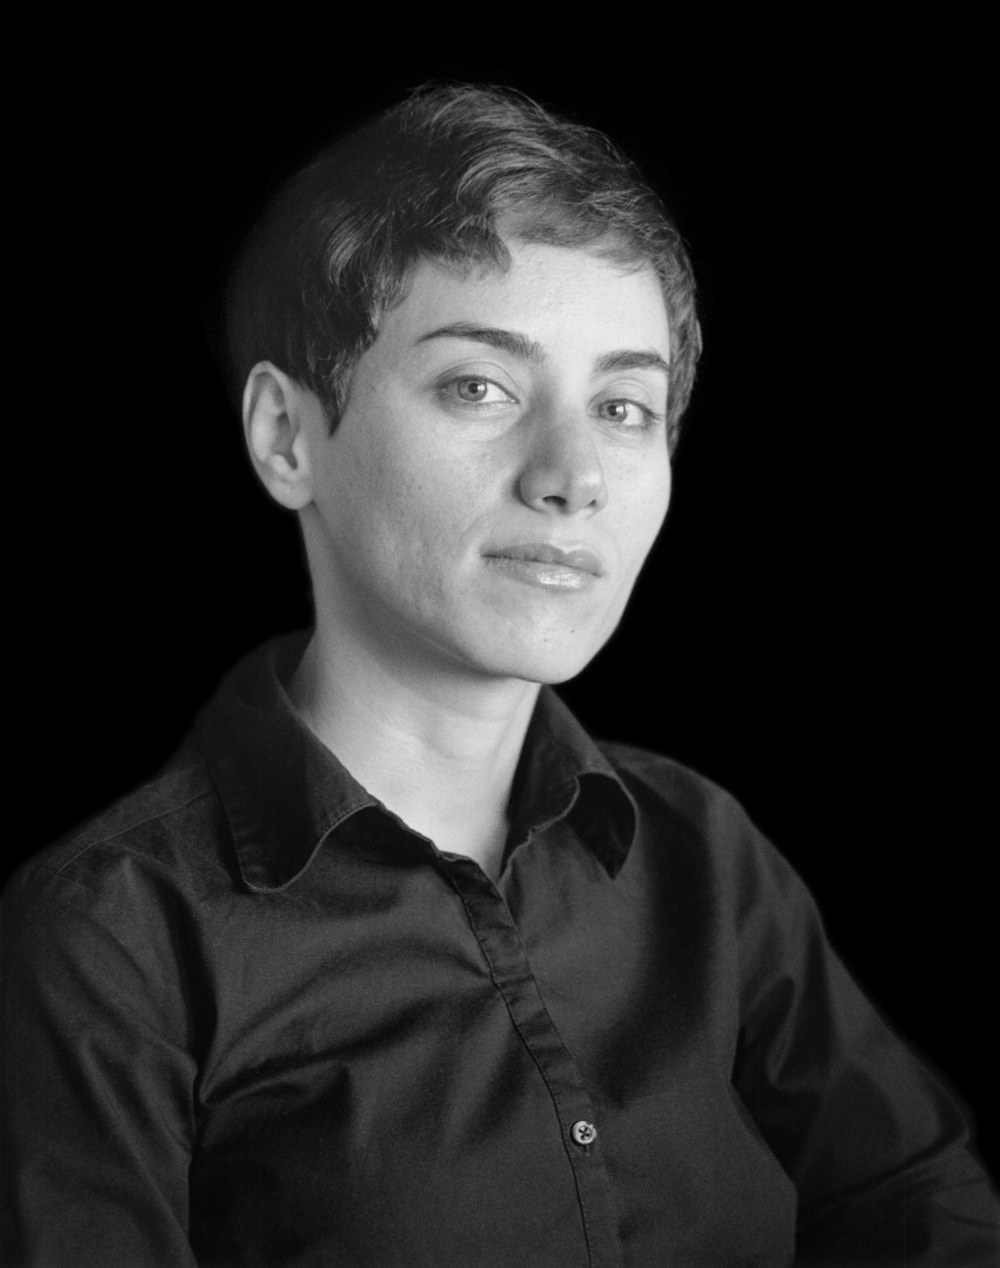
\includegraphics[width=0.4\textwidth]{static/maryam.jpg} \\
    \vspace{.8cm}
    \tiny{\url{www.newyorker.com/tech/annals-of-technology/maryam-mirzakhanis-pioneering-mathematical-legacy}}

    \end{center}
\end{frame}

\begin{frame}
    \begin{center}
    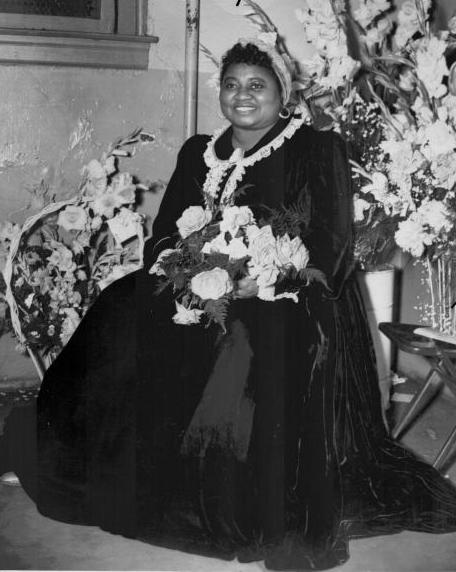
\includegraphics[width=0.40\textwidth]{static/hattie.jpg} \hspace{10pt}
    
\includegraphics[width=0.40\textwidth, height=.505\textwidth]{static/ali.jpg}
    \vspace{.8cm}

    \tiny{\url{en.wikipedia.org/wiki/List_of_black_Academy_Award_winners_and_nominees}
    \url{www.eonline.com/news/836150/}}

    \end{center}
\end{frame}

\begin{frame}
    \centering
    \LARGE \textbf{EQUALITY} \textcolor{orange}{VS} \textbf{EQUITY}
\end{frame}

\begin{frame}
    \begin{center}
    \begin{minipage}{.5\textwidth}
        \LARGE{EQUALITY}
    \end{minipage}
    \begin{minipage}{.3\textwidth}
        \normalsize{[ih-kwol-i-tee]}
    \end{minipage}
    \vspace{.5cm}

    \hspace{-8cm} \normalsize{[noun]}\\
    \end{center}
    \hspace{.8cm} \normalsize{1. the state of being equal, especially in status, or}

    \hspace{.8cm} \normalsize{opportunities.}
    \vspace{.5cm}

    \begin{center}
    \begin{minipage}{.5\textwidth}
        \LARGE{EQUITY}
    \end{minipage}
    \begin{minipage}{.3\textwidth}
        \normalsize{[ek-wi-tee]}
    \end{minipage}
    \vspace{.5cm}

    \hspace{-8cm} \normalsize{[noun]}\\
    \end{center}
    \hspace{.8cm} \normalsize{1.  the quality of being fair and impartial.} \\ 
\end{frame}

\begin{frame}
    \begin{center}
        \includestandalone[width=.45\textwidth]{static/race}
    \end{center}
\end{frame}

\begin{frame}
    \begin{center}
        \includestandalone[width=.45\textwidth]{static/race_equity}
    \end{center}
\end{frame}

\begin{frame}
    \begin{center}
    \begin{minipage}{.5\textwidth}
        \LARGE{BIAS}
    \end{minipage}
    \begin{minipage}{.3\textwidth}
        \normalsize{[bahy-uhs]}
    \end{minipage}
    \vspace{.5cm}

    \hspace{-8cm} \normalsize{[noun]}\\
    \end{center}
    \hspace{.8cm} \normalsize{1. a particular tendency, trend, inclination, feeling,}

    \hspace{1cm} \normalsize{or opinion, especially one that is preconceived or}

    \hspace{1cm} \normalsize{unreasoned.}
\end{frame}

\begin{frame}
    \begin{center}
        \textbf{\Large{\textcolor{orange}{UNCONSCIOUS} BIAS}}
    \end{center}
\end{frame}

\begin{frame}
    \begin{center}
        \textbf{\Large{\textcolor{orange}{AFFINITY} BIAS}}
        \vspace{.5cm}

        
\includegraphics[width=.1\textwidth]{static/person.png}
        
\includegraphics[width=.1\textwidth]{static/person.png}
    \end{center}
\end{frame}

\begin{frame}
    \begin{center}
        \textbf{\Large{\textcolor{orange}{HALO} EFFECT}}
        \vspace{.5cm}

        
\includegraphics[width=.1\textwidth]{static/halo.png}
    \end{center}
\end{frame}

\begin{frame}
    \begin{center}
        \textbf{\Large{\textcolor{orange}{HORNS} EFFECT}}
        \vspace{.5cm}

        
\includegraphics[width=.1\textwidth]{static/horn.png}
    \end{center}
\end{frame}

\begin{frame}
    \begin{center}
        \textbf{\Large{\textcolor{orange}{ATTRIBUTION} BIAS}}
        \vspace{.5cm}

        
\includegraphics[width=.1\textwidth]{static/scale.png}
    \end{center}
\end{frame}

\begin{frame}
    \begin{center}
        \textbf{\Large{\textcolor{orange}{CONFORMITY} BIAS}}
        \vspace{.5cm}

    
\includegraphics[width=.1\textwidth]{static/thought-balloon.png}
    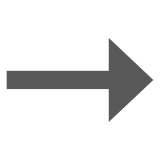
\includegraphics[width=.1\textwidth]{static/arrow.png}
    
\includegraphics[width=.1\textwidth]{static/people.png}
    
\includegraphics[width=.1\textwidth]{static/people.png}
    \end{center}
\end{frame}

\begin{frame}
    \begin{center}
    \Large \textbf{EFFECT OF \textcolor{orange}{UNCONSCIOUS} BIAS IN HIERARCHICAL SYSTEM}
    \end{center}
\end{frame}

\begin{frame}
    \centering
    \LARGE{\textbf{\textcolor{orange}{HIERARCHICAL SYSTEM}}} \\
    \vspace{1cm}
    \begin{minipage}{0.7\textwidth}
        \includestandalone[width=\textwidth]{static/states}
    \end{minipage}\hspace{1cm}
\end{frame}

\begin{frame}
    \centering
    \LARGE{\textbf{\textcolor{solarizedBase03}{HIERARCHICAL SYSTEM}}} \\
    \vspace{1cm}
    \begin{minipage}{.7\textwidth}
        \hspace{-.5cm}\includestandalone[width=\textwidth]{static/competence}
    \end{minipage}
\end{frame}

\begin{frame}[fragile]
    \begin{minted}
        [
        autogobble=true,
        framesep=2mm,
        fontsize=\tiny,
        bgcolor=DarkGray,
        ]
        {python}
>>> import hierarchical as hrcy
>>> import numpy as np
>>> import scipy.stats

>>> competence_distribution = scipy.stats.uniform(0, 1)
>>> retirement_rate = 0.2
>>> capacities = [3, 2, 1]

>>> np.random.seed(0)
>>> states = list(hrcy.states.get_competence_states(
...         capacities, competence_distribution, retirement_rate)
... )

>>> for level_index, level in enumerate(states[6]):
...    print(f"Level {2 - level_index}")
...    for individual in level:
...        print(
...            f"""-|type {individual.individual_type} with
...    competence {individual.competence:.3f} retirement {individual.retirement_date:.3f}"""
...        )
Level 2
-|type 0 with
    competence 0.438 retirement 0.445
-|type 1 with
    competence 0.964 retirement 0.097
-|type 1 with
    competence 0.792 retirement 0.151
Level 1
-|type 0 with
    competence 0.360 retirement 0.115
-|type 1 with
    competence 0.698 retirement 0.012
Level 0
-|type 0 with
    competence 0.209 retirement 0.035
    \end{minted}
\end{frame}

\begin{frame}
    \centering
    \LARGE{\textbf{\textcolor{orange}{RETIREMENT}}} \\
    \vspace{1cm}

    \hspace{-.5cm}
    \begin{minipage}{0.29\textwidth}
        \includestandalone[width=1.3\textwidth]{static/full_system}
    \end{minipage}\hfill
    \begin{minipage}{.29\textwidth}
        \includestandalone[width=1.3\textwidth]{static/retirement_states}
    \end{minipage}\hfill
    \begin{minipage}{.29\textwidth}
        \includestandalone[width=1.3\textwidth]{static/retired_state}
    \end{minipage}
\end{frame}

\begin{frame}
    \centering
    \LARGE{\textbf{\textcolor{orange}{PROMOTION}}} \\
    \vspace{1cm}

    \hspace{-.5cm}
    \begin{minipage}{0.29\textwidth}
        \includestandalone[width=1.3\textwidth]{static/retired_state}
    \end{minipage}\hfill
    \begin{minipage}{.29\textwidth}
        \includestandalone[width=1.3\textwidth]{static/promotion_states}
    \end{minipage}\hfill
    \begin{minipage}{.29\textwidth}
        \includestandalone[width=1.3\textwidth]{static/promoted_states}
    \end{minipage}
\end{frame}

\begin{frame}
    \centering
    \vspace{.5cm}
    \LARGE{\textbf{\textcolor{orange}{HIRING}}} \\
    \vspace{.3cm}

    \hspace{-.5cm}
    \begin{minipage}{0.29\textwidth}
        \includestandalone[width=1.3\textwidth]{static/promoted_states}
    \end{minipage}\hfill
    \begin{minipage}{0.29\textwidth}
        \vspace{.65cm}\includestandalone[width=1.3\textwidth]{static/hire_states}
    \end{minipage}\hfill
    \begin{minipage}{0.29\textwidth}
        \includestandalone[width=1.3\textwidth]{static/hired_states}
    \end{minipage}
\end{frame}

\begin{frame}
    \centering
    \begin{columns}
        \begin{column}{.45\textwidth}
        \centering
        \LARGE{\textcolor{orange}{\textbf{RETIREMENT}}} \\
        \vspace{.75cm}

        \LARGE{\textcolor{orange}{\textbf{HIRING}}} \\
        \vspace{.75cm}

        \LARGE{\textcolor{orange}{\textbf{PROMOTION}}} \\
        \end{column}
        \hspace{-1cm}
        \begin{column}{.25\textwidth}
        
\includegraphics[width=.5\textwidth]{static/retirement.pdf} \\
        \includegraphics[width=.5\textwidth]{static/hire.pdf} \\
        
\includegraphics[width=.5\textwidth]{static/promotion.pdf} \\
        \end{column}
    \end{columns}
\end{frame}

\begin{frame}
    \centering
        \includestandalone[width=.7\textwidth]{static/before_promotion}
\end{frame}

\begin{frame}
    \centering
        \includestandalone[width=.7\textwidth]{static/promotion}
\end{frame}

\begin{frame}[fragile]
    \begin{center}
    \begin{minted}
        [
        autogobble=true,
        framesep=2mm,
        fontsize=\scriptsize,
        bgcolor=DarkGray,
        ]
        {python}
>>> capacities = [9, 6, 2, 1]

>>> competence_distribution = scipy.stats.uniform(0, 1)
>>> retirement_rate = 0.2
>>> lmbda = [10, 10]
    \end{minted}
\end{center}
\end{frame}

\begin{frame}[fragile]
    \begin{center}
    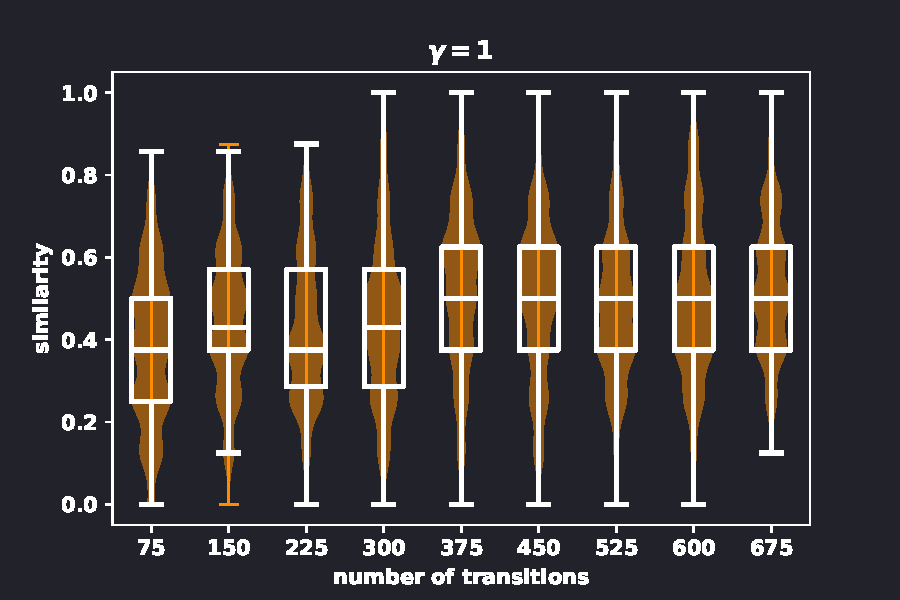
\includegraphics[width=.7\textwidth]{static/average_similarity_ratio.pdf}
    \end{center}
\end{frame}

\begin{frame}
    \centering
    \LARGE \textbf{UNCONSCIOUS \textcolor{orange}{BIAS}} \\
    \vspace{1cm}

    \LARGE \textbf{\textcolor{orange}{AFFINITY} BIAS}
\end{frame}

\begin{frame}
    \centering
        \includestandalone[width=.7\textwidth]{static/competence_promotion}
\end{frame}

\begin{frame}[fragile]
    \begin{center}
    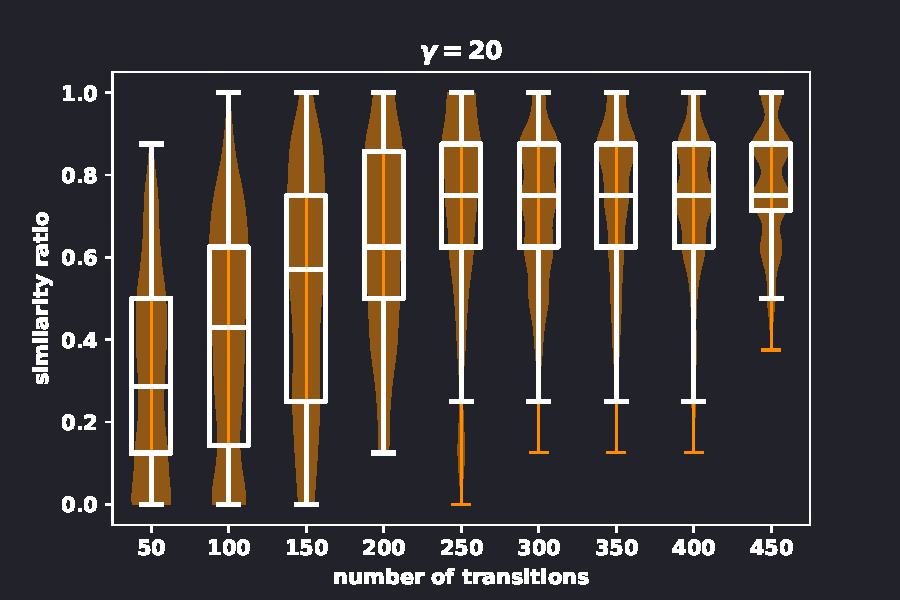
\includegraphics[width=.7\textwidth]{static/high_similarity_ratio.pdf}
    \end{center}
\end{frame}

\begin{frame}[fragile]
    \begin{minipage}{.49\textwidth}
    \includestandalone[width=\textwidth]{static/meritocracy_competence}
    \end{minipage}
    \begin{minipage}{.49\textwidth}
        \vspace{-.1cm} \includestandalone[width=\textwidth]{static/affinity_competence}
    \end{minipage}
\end{frame}

\begin{frame}[fragile]
    \centering
        \vspace{-1cm}
        \includestandalone[width=\textwidth]{static/affinity_competence_}
\end{frame}

\begin{frame}
    \begin{center}
    \Large \textbf{HOW MUCH \textcolor{orange}{WORSE} IS THE SYSTEM BECAUSE OF AFFINITY BIAS?}
    \end{center}
\end{frame}

\begin{frame}[fragile]
    \begin{center}
        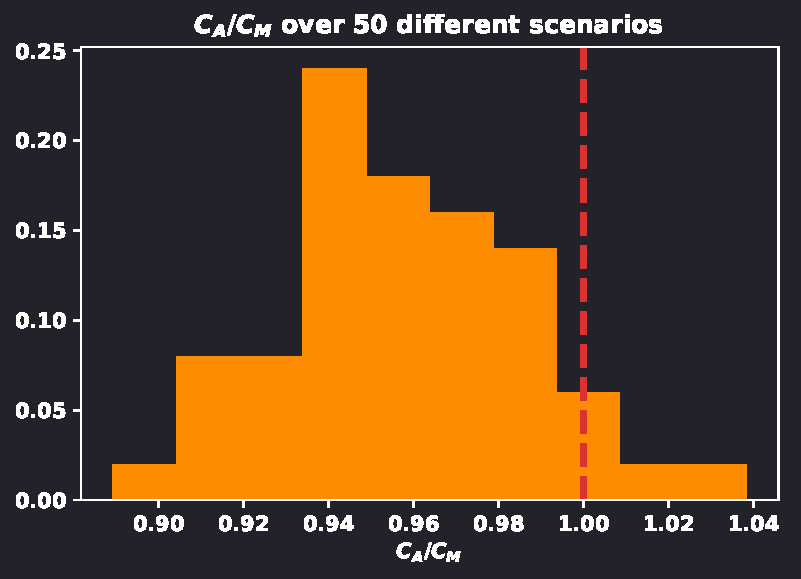
\includegraphics[width=.7\textwidth]{static/ratio_one_to_twenty.pdf}
    \end{center}
\end{frame}

\begin{frame}[fragile]
    \begin{center}
    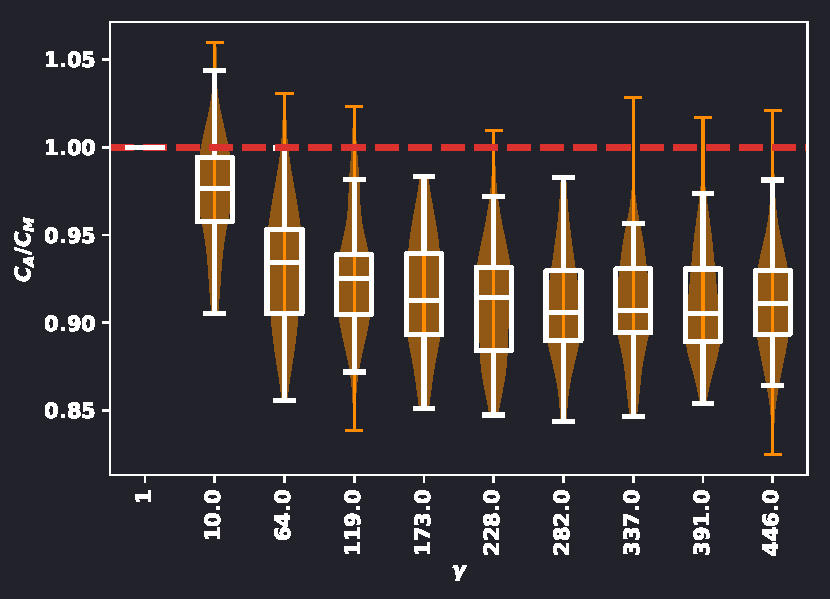
\includegraphics[width=.7\textwidth]{static/ratio_over_gammas.pdf}
    \end{center}
\end{frame}

% \begin{frame}
%         \centering
%         \animategraphics[loop,
%                          controls,
%                          width=\textwidth]{1}{static/gif/}{0}{1999}
% \end{frame}

\begin{frame}[fragile]
    \begin{center}
    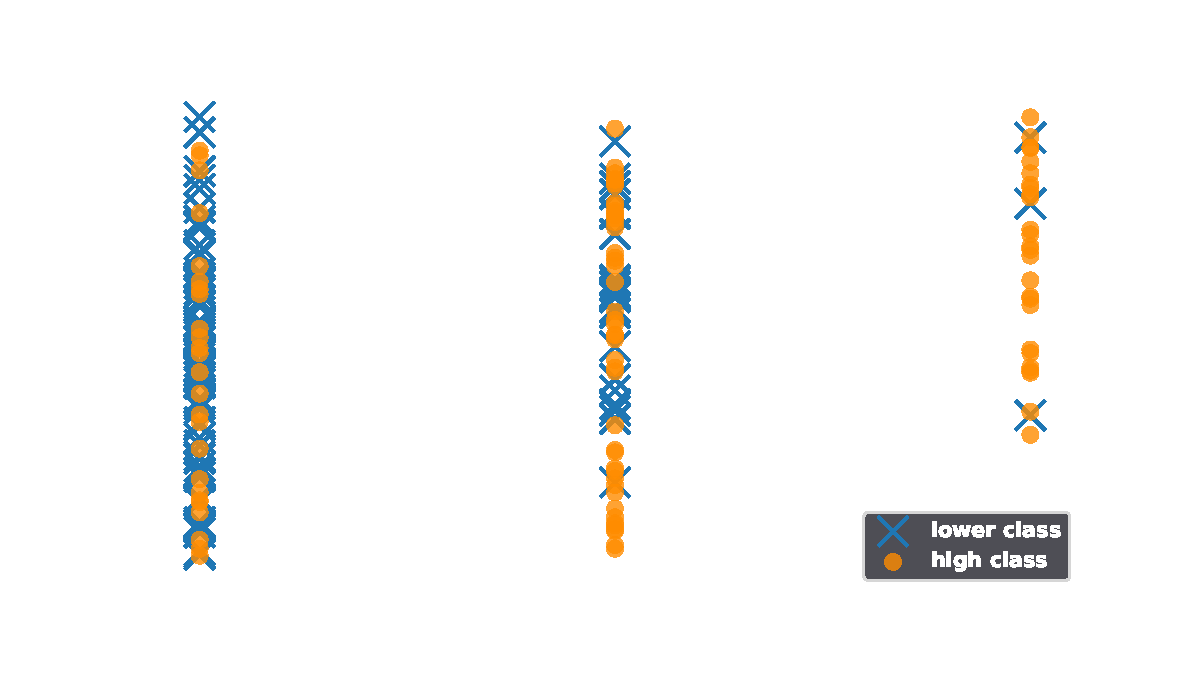
\includegraphics[width=.7\textwidth]{static/exit_levels.pdf}
    \end{center}
\end{frame}

\begin{frame}
    \centering
    \LARGE \textbf{ANSWERS?}
\end{frame}

\begin{frame}
    \centering
    \LARGE \textbf{BE \textcolor{orange}{AWARE} OF YOUR UNCONSCIOUS BIAS}
\end{frame}

\begin{frame}
    \centering
    \LARGE \textbf{BE \textcolor{orange}{AN ALLY}}
\end{frame}

\begin{frame}
    \centering
    \LARGE \textbf{DO \textcolor{orange}{NOT} BE LAZY}
\end{frame}

\begin{frame}
    \begin{center}
    \faTwitter @NikoletaGlyn \\
    \faTwitter @drvinceknight \\
    
    \vspace{1cm}
    \end{center}

    \footnotesize
    $\bullet$ https://nikoleta-v3.github.io \\
    $\bullet$ \url{vknight.org/unpeudemath/math/2017/11/10/the-fallacy-of-meritocracy.html} \\
    \faGithub  \ \url{github.com/drvinceknight/HierarchicalPromotion}
\end{frame}

\end{document}

